\documentclass[12pt]{article}
\setlength{\textwidth}{17cm}
\setlength{\textheight}{24cm}
\setlength{\topmargin}{-2cm}
\setlength{\footskip}{1cm}
\setlength{\evensidemargin}{0cm}
\setlength{\oddsidemargin}{0cm}
\setlength{\parindent}{0cm}

%\usepackage{allrunes}
\usepackage{amsmath}
\usepackage[hungarian]{babel}
\usepackage[T1]{fontenc}
\usepackage[utf8]{inputenc}
\usepackage{fixltx2e}
\usepackage{multirow}

\usepackage[hyphens]{url}
\usepackage[unicode,colorlinks=true,breaklinks]{hyperref}
%\usepackage[dvips]{hyperref}
%should display links, but it does not work with \H accent
%and formulas in section titles

\hypersetup{colorlinks,linkcolor=blue,urlcolor=magenta,citecolor=magenta}
%Breaks long url`s in text, while keeping it one link:

\usepackage{amsfonts}
\usepackage{amsthm}
\usepackage{amssymb}


\theoremstyle{plain}
\usepackage{graphicx}

%\usepackage{gensymb}
\usepackage{float}

% For bra-ket notation
\usepackage{braket}

%% New commands
\newcommand{\dd}{\textrm{d}}

%% Pauli matrices
\newcommand{\sigx}{\sigma_x}
\newcommand{\sigy}{\sigma_y}
\newcommand{\sigz}{\sigma_z}

\newcommand{\paulix}{
    \left( \begin{array}{cc}
        0 & 1 \\
        1 & 0
    \end{array}
    \right)
}

\newcommand{\pauliy}{
    \left( \begin{array}{cc}
        0 & -i \\
        i & 0
    \end{array}
    \right)
}

\newcommand{\pauliz}{
    \left( \begin{array}{cc}
        1 & 0 \\
        0 & -1
    \end{array}
    \right)
}


\begin{document}
\title{5. tétel}
\author{Furuglyás Kristóf}

\maketitle


\newpage
\begin{abstract}
    Fraktáldimenzió, önhasonló matematikai fraktálok, természetben előforduló fraktálok, sejtautomaták.
\end{abstract}

\section{Fraktáldimenzió}
Mindennapi objektumoknál megfigyelhető, hogy ha egyre kisebb skálán vizsgáljuk őket, az egyes tulajdonságaik konvergálnak egy adott értékhez. Fraktálok esetében azonban a kisebb felbontás nem eredményez konvergenciát; \textbf{a fraktálok határai} ugyanis végtelenül "gyűröttek" vagy "szakadásosak", azaz \textbf{nem-differenciálhatóak}. Továbbá, a fraktálok másik fontos tulajdonsága, hogy \textbf{önhasonlók} -- azaz különböző nagyítás mellett nézve ugyanazt az alakzatot látjuk kibontakozni. A természetben előforduló fraktálok például a \textbf{szigetek partvonalai vagy a hegyek felszíne}. Előfordulhatnak még \textbf{növekedésből származó fraktálok} is, mint például az a \textbf{növények gyökérzete vagy épp a keringési rendszer}. Ilyenkor az elégazó struktúrák valamilyen \textbf{növekedési instabilitás} váltja ki. \\

Megmérve bármilyen $d$ dimenziós test a térfogatát különböző $l$ oldalhosszúságú szintén $d$ dimenziós (tehát $l^d$ térfogatú) kockákkal, és feltételezve, hogy ekkor a lefedéshez szükséges kockák száma $N \left( l \right)$, a test téfogata: 

\begin{equation}
V \left( l \right) =  N \left( l \right) \cdot l^d.
\end{equation}

Hétköznapi objektumoknál ha $l \rightarrow 0$, akkor $V \left(l \right)$ gyorsan konvergál egy adott értékhez. Azonban \textbf{fraktálok} esetében ha $l \rightarrow 0$, akkor $\mathbf{V \left(l \right) \rightarrow 0}$! Ugyanakkor ezzel egyidőben a $d-1$ dimenziós $S \left( l\right)$ \textbf{felszíne pedig divergál}: $\mathbf{ S \left( l \right) \rightarrow \infty}$. \\

A geomatriai (matematikai) fraktálok:
\begin{itemize}
	\item olyan \textbf{önhasonló} geometriával rendelkező formák,
	\item ahol az önhasonlóság \textbf{tetszőleges iteráción keresztül} fennáll, 
	\item és a lefedéshez szükséges $l$ élhosszúságú dobozok $N \left( l \right) $ száma \textbf{nemtriviálisan skálázódik}:
		\begin{equation}
					N \left( l \right) \sim l^{-D},
		\end{equation}
	ahol $D$ egy pozitív, nem egész szám, amely az objektum törtdimenziója, fraktáldimenziója.
\end{itemize}

Az előbbiek alapján a két oldal logaritmusát véve definiálhatjuk a fraktál \textbf{box-counting dimenzióját}:
\begin{equation}
D_B = \lim_{l \rightarrow 0 } \frac{\ln N \left( l\right) }{\ln \left(1/l\right)}.
\end{equation}
Ugyanez érvényes akkor is, \textbf{ha a fraktál növekvő}, és annak lineáris hosszát $L$-lel jelöljük:
\begin{equation}
D_B = \lim_{L \rightarrow \infty } \frac{\ln N \left( L\right) }{\ln L}.
\end{equation}



\begin{figure}[H]
    \begin{center}
    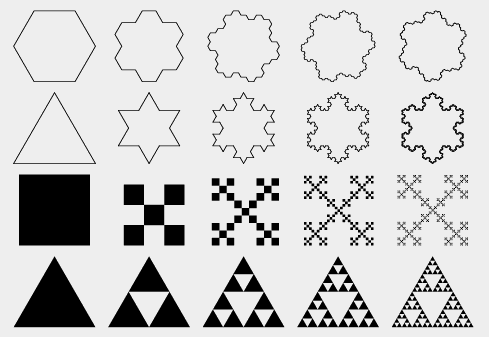
\includegraphics[width=0.5\textwidth]{media/fractal_pelda.png}
    \caption{Példa fraktálokra különböző iterációk után. Lehet látni, hogy változik a térfogat és a felszín aránya. } 
    \label{fig:fractal_peldak}
    \end{center}
\end{figure}

\subsection{Műveletek}

A fraktálokkal, mint matematikai objektumokkal műveleteket is végezhetünk:
\begin{itemize}
	\item \textbf{Projekció}: $d$ dimenziós euklidészi térbe ágyazott $D$ dimenziós fraktált projektálunk egy $d_s$ dimenziós szintér eklidészi altérre:
	\begin{itemize}
		\item ha $d_s>D$, akkor a projekció dimenzió nem változik, $D_p = D$,
		\item ha $d_s<D$, akkor a projekció kitölti a rendelkezésre álló teret, $D_p = d_s$. Tehát $\mathbf{D_p =\max \left(D, d_s\right) }$ .
	\end{itemize}  
	\item \textbf{Metszet I.} : ha vesszük egy $d$ dimenziós euklidészi térbe ágyazott $D$ dimenziós fraktál és egy $d-m$ dimenziós szintén euklidészi tér metszetét, akkor a metszet dimenziója $\mathbf{D_i = D-m}$ lesz.
	\item \textbf{Metszet II.} : két fraktál metszetének dimenzióját a részecskék sűrűségéből tudjuk kiszámolni:
	\begin{itemize}
		\item egy $L$ lineáris hosszúságú szakaszon az $A$ fraktál részecskéinek sűrűsége $\sim \frac{L^{D_A}}{L^d}$, B-nek hasonlóképp,
		\item mivel a két fraktál részecskéinek eloszlása független egymástól, az együttes sűrűség $\sim \frac{L^{D_A}}{L^d} \cdot \frac{L^{D_B}}{L^d}$, az összes részecskét pedig a teljes térre nézzük -- $N_{A \cap B} \left(L \right) \sim \frac{L^{D_A} L^{D_B}}{L^d}$,
		\item tehát a dimenzió leolvasható: $\mathbf{D_{A \cap B} = D_A + D_B - d}$.
	\end{itemize}
	\item \textbf{Unió}: két fraktál uniójának dimenzióját a nagyobbik dimenziójú fraktál fogja megadni, azaz $\mathbf{D_{A\cup B} = \max \left( D_A, D_B \right) }$.
	\item \textbf{Szorzat}: két fraktál szorzatának dimenziója a fraktálok dimenziójának összege, azaz $\mathbf{D_{AB} = D_A + D_B}$.

\end{itemize}

\subsection{Típusok}

\paragraph{Determinisztikus fraktál}
Egy fraktál determinisztikus, ha önhasonló rekurzióval generálódik -- azaz vagy kicseréljük a részeit önmaga lekicsinyített képével vagy önmaga felnagyított képével. Ezekre tökéletes példát mutat a \ref{fig:fractal_peldak}. ábra. Például, ha harmadik sorban egységoldalúnak vesszük az első ábrát és a mellette lévőket felskálázzuk úgy, hogy az egyes négyzetek oldalai rendre egységhosszúak legyenek, akkor egy növekvő fraktált kapunk. Ennek a fraktálnak a lineáris mérete a háromszorosára, kvázi "területe", azaz a lefedéshez szükséges négyzetek száma pedig az ötszörösére nő. Ezek alapján a fraktál dimenziója:

\begin{equation}
D = \lim_{L \rightarrow \infty } \frac{\ln N \left( L\right) }{\ln L} = \lim_{k \rightarrow \infty} \frac{ \ln \left( 5 ^k\right) }{ \ln \left( 3^k\right)} = \frac{\ln 5}{ \ln 3} = 1.465\dots
\end{equation}

\begin{figure}[H]
    \begin{center}
    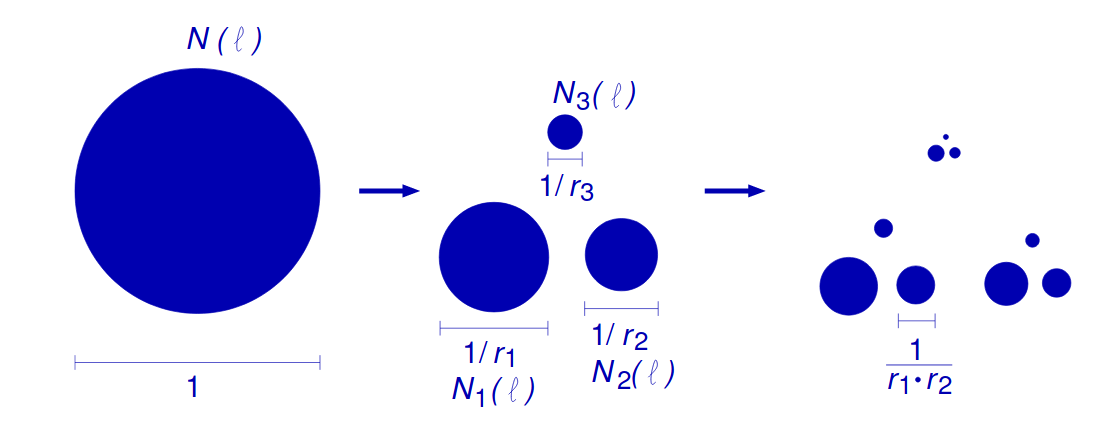
\includegraphics[width=0.5\textwidth]{media/fractal_non_uni.png}
    \caption{Példa non-uniform fraktálra. } 
    \label{fig:fractal_non_uni}
    \end{center}
\end{figure}

Előfordulhat azonban, hogy nem egyenletes a másolatok nagysága -- lásd \ref{fig:fractal_non_uni}. ábra. Ekkor ha $q$ különböző másolatot készítünk ($r_1, r_2, \dots, r_q$), akkor az összes lefedéshez szükséges négyzet az elsóbb fraktálokból jön: $N \left( l \right) = \sum_{i = 1}^q N_i\left( l\right)$. Az önhasonlóság miatt $ N\left( l\right) = N_i\left( l / r_i\right)$. A fraktál definíciójából jön, hogy $N_i \left( l\right) = N \left( lr_i \right) \sim \left( lr_i \right)^{-D_B}$. Visszahelyettesítve $N \left( l \right) = \sum_{i = 1}^q N_i\left( l\right) =\sum_{i = 1}^q \left( lr_i \right)^{-D_B} \sim l^{-D_B}$, tehát a dimenzióra egy implicit egyenletet kapunk: $\sum_{i_1}^q r_i^{-D_B} = 1$.






\paragraph{Szotochasztikus fraktálok}
Hasonlóképp, mint a determinisztikus fraktáloknál, itt is van egy önhasonló rekurzió, mellyel generálódik a fraktál, azonban ekkor bejön továbbá egy random tényező. Ha a random tényező nem befolyásolja fraktál méretét, csak a struktúráját, akkor a fraktál box-counting dimenziója ugyanaz, mint a determinisztikus esetben -- lásd \ref{fig:stoch_cantor}. ábra.

\begin{figure}[H]
    \begin{center}
    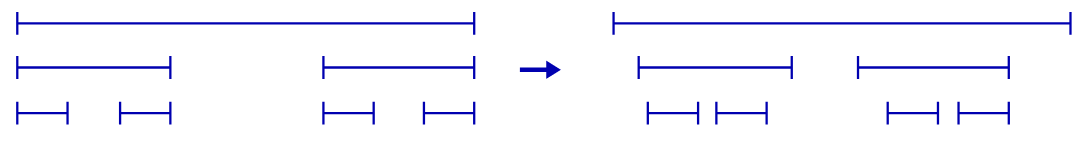
\includegraphics[width=0.5\textwidth]{media/stoch_cantor.png}
    \caption{Sztochasztikus Cantor halmaz. Bal oldalon determinisztikus, jobb oldalon sztochasztikus formában. Észrevehető, hogy a lefedéshez szükséges négyzetek száma $(N \left( l \right))$ nem változik.} 
    \label{fig:stoch_cantor}
    \end{center}
\end{figure}

\paragraph{Random fraktálok}

\begin{figure}[H]
    \begin{center}
    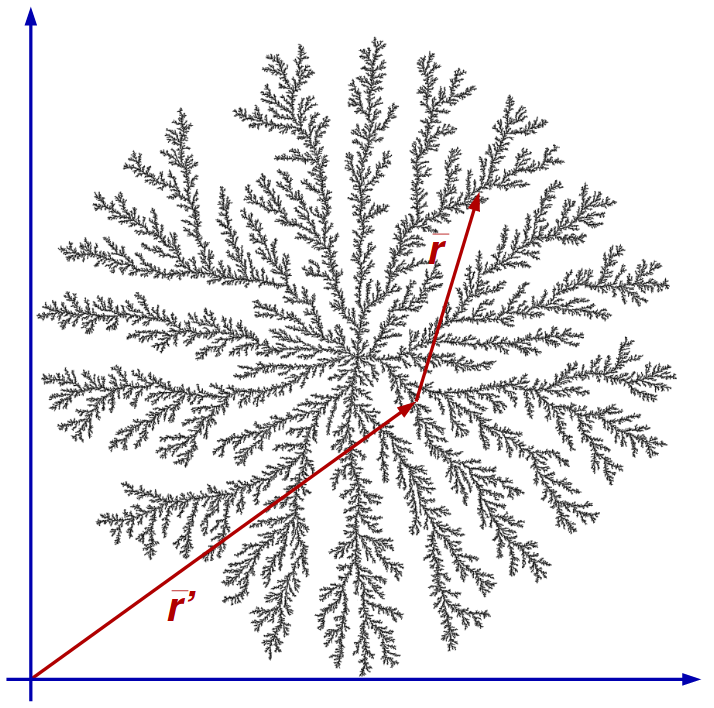
\includegraphics[width=0.5\textwidth]{media/dla_frac.png}
    \caption{Diffúzió-limitált növekedés következtében kialakult random fraktálszerkezet. Ilyen lehet például egy baktériumtelep, vagy elektromos áram elvezetése fában.}
    \label{fig:dla_frac}
    \end{center}
\end{figure}

\begin{figure}[H]
    \begin{center}
    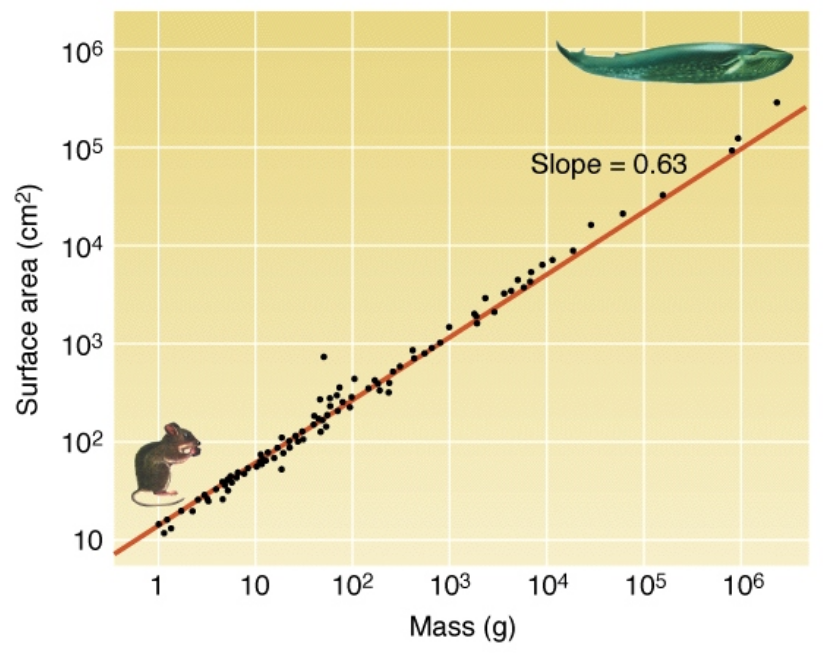
\includegraphics[width=0.5\textwidth]{media/allometry.png}
    \caption{Az állatok tömegének és felületének összefüggése log-log skálán.}
    \label{fig:allometry}
    \end{center}
\end{figure}

A legtöbb, természetben előforduló fraktál ilyen. Ekkor nincsen iterációs szabály, és emiatt a dimenzió kiszámítása is bonyolulttá válhat, ezért célszerűbb a sűrűség-korrelációs függvényt vizsgálni:

\begin{equation}
C\left( \vec{\mathbf{r}} \right) = \frac{1}{V} \sum_{\vec{\mathbf{r'}}} \rho \left(\vec{\mathbf{r + r'}} \right)\rho \left(\vec{\mathbf{r'}} \right),
\end{equation}
ahol $V$ a térfogat, a szumma a tér minden pontjára vonatkozik, a $\rho \left(\vec{\mathbf{r}} \right)$ pedig a sűrűségfüggvény, mely $=1$ ha a $\vec{\mathbf{r}} $ pontban van fraktál és $=0$ egyébként -- \ref{fig:dla_frac}. ábra. A sűrűség-korrelációs függvény izotróp testek esetében csak a sugártól függ, és amíg hétköznapi objektumokra a lépcsőfüggvény, kristályrácsra pedig diszkrét vonalak, addig fraktáloknál skálázódik:

\begin{equation}
C\left(r\right) \sim r^{-\alpha}.
\end{equation}

A skálázódásra példa lehet \href{https://en.wikipedia.org/wiki/Zipf's_law}{Zipf törvénye}, illetve a biológiában az allometria (élőlények tulajdonságia közötti arány). A skálázódásból fakadóan kiszámítható a fraktálhoz szükséges négyzetek száma:

\begin{equation}
N \left( L \right)  \sim \int_0^L C \left( r \right) d^dr \sim L^{d-\alpha},
\end{equation}

melyből leolvasható, hogy $D = d- \alpha$. 

\section{Természetben előforduló fraktálok}
A természetben előforduló fraktálok többsége növekvő fraktál. Ebben a fejezetben erre fogunk példákat nézni.


\subsection{Random mozgás}
Négyzetrácson történő mozgást nézünk, ahol az egyen irányokba történő elmozdulás valószínűsége ugyanakkora. Ekkor egy dimenzióban az elmozdulásnak $i$ lépés után $(x_i)$ a várható értéke nulla, $\left< x_i\right>  = 0$., szórása egy, $\sigma\left( x_i\right) = 1$. Az pozíció $\left( x \right)$ a centrális határeloszlás-tétel következtében egy $\mu = 0$ várhatóértékű és $\sigma = \sqrt{t} $ szórású normális eloszlást fog követni:

\begin{equation}
\rho \left( x\right) = 	\frac{1}{\sqrt{1\pi t}} \exp^{-\frac{x^2}{2}}.
\end{equation}
Amelyből kifolyólag az átlagos elmozdulás az origótól az időnek a gyökével egyenlő:

\begin{equation}
R = \sqrt{\left< x^2\right>} = \sqrt{t}.
\end{equation}

$d= 2,3$ dimenzióban feltételezzük, hogy az irányok egymástól függetlenek, így több normális eloszlás összege $\chi$ eloszlást fog követni, melyből megkapható, hogy az átlagos távolság arányos:

\begin{equation}
\left< R \right> = \sqrt{t} \sqrt{\frac{2}{d}} \frac{\Gamma \left( \frac{d+1}{2}\right)}{\Gamma \left( d/2 \right)} \Longrightarrow \left< R \right> \sim \sqrt{t}
\end{equation}

Hogyan lesz ebből fraktál? Ha minden pontot, ahol a részecskénk járt, kitöltünk, a teljes objektum fraktál-struktúrát fog mutatni, feltéve, hogy $ d \geqslant 3 $.



\subsection{Aggregátumok, perkoláció}
Az aggregátumok olyan objektumok, melyben elemi blokkok kapcsolódnak egymáshoz. A perkoláció pedig az anyagnak akadályokkal teli, porózus közegben történő mozgását jelenti. Jelen esetben mindvégig csak olyan objektumokról beszélünk, melyben az elemi blokkok megkülönböztethetetlenek, teljesen ugyanazok. Négyzetrácson (diszkrét térben) a szomszéd jelentheti az egy egységen belüli lépéseket (azaz 2 dimenzióban 4 szomszéd például) vagy tekinthetjük az átlós helyeket is (2 dimenzióban 9 szomszéd). Valós (folytonos) térben a szomszédoknak az adott távolságon belüli pontokat értjük, ugyanakkor itt figyelembe vesszük, hogy azok között kölcsönhatás lehet. \\

Aggregációnál általában egy maghoz kapcsolódnak a blokkok egy sztochasztikus folyamat révén. Ez kétféleképpen valósulhat meg: 1) elindítunk random pozícióból egy részecskét és az csatlakozik valahol a klaszterhez, avagy 2) kiválasztunk egy a klaszternek szomszédos véletlenszeű pozíciót és azt szintén random paraméterek alapján vagy kitöltjük, vagy nem. Pszeudo-random paraméter például a hőmérséklet-szerű paraméterek vagy több más paraméter összessége. \\

\paragraph{Lokális modell} A lokális modellben a helyszín kitöltése csakis önmagától (betöltött-e vagy sem) és a többi szomszédtól függhet (diagonális megengedett) -- ilyenek például a sejtautomaták és a diffúzió-limitált növekedés alapú baktériumtelepek is. A lokális modellben elöfordulhatnak egymástól független klaszterek is, másnéven rács-állatkák (lattice animals) -- lásd \ref{fig:lattice_animals}. ábra. A rács-állatkák típusa (szimmetriák megléte (forgatás és/vagy tükrözés)), illetve gyakorisága jellemző az iterációs módszerre -- erről bövebben később a \ref{sec:cellular_automatons}. fejezetben. 

\begin{figure}[H]
    \begin{center}
    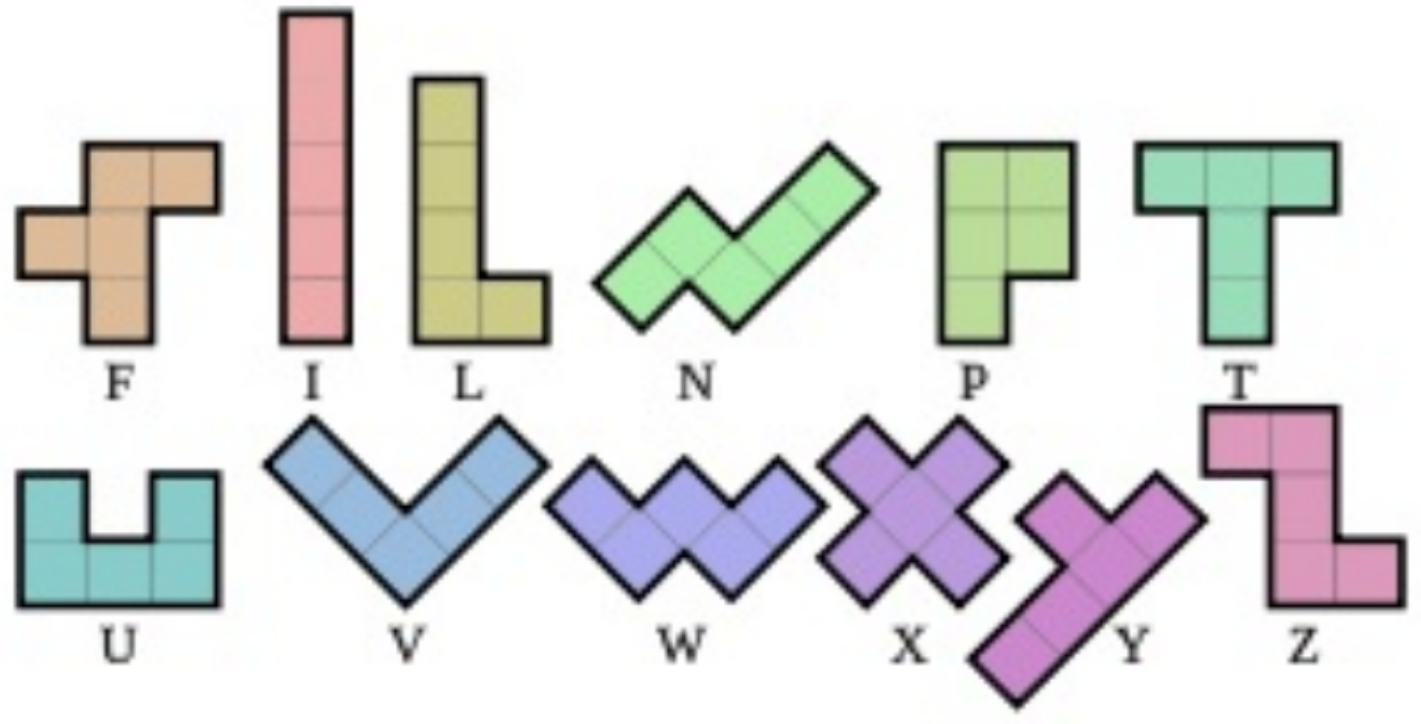
\includegraphics[width=0.5\textwidth]{media/lattice_animals.png}
    \caption{Rács-állatkák két dimenzióban. } 
    \label{fig:lattice_animals}
    \end{center}
\end{figure}



\paragraph{Nemlokális modell}
A nemlokális modellben azonban megengedhetjük a távolhatást, azaz a távoli részecskék közötti kölcsönhatást -- erre tökéletes példa az \href{https://en.wikipedia.org/wiki/Abelian_sandpile_model}{ábeli homokdomb modell}. Ebben -- értelemszerűen -- a lokális randomitás helyett a globális lesz jelen. \\

A perkolációs modell esetében egy véges rács minden pontjához rendelünk valami random számot (0 és 1 között), majd  egy $p$ határérték (\textit{valószínűség}) alatt feltöltjük azokat. Ekkor lehet vizsgálni a legnagyobb klaszter méretét, melynek keletkezése egy bizonyos $p_c$ kritikus valószínúségnél következik be. Perkolációra példa a természetben a szivacsban, falban vagy kőben történő folyadékterjedés. 

\subsection{Diffúzió-limitált növekedés}
A diffúzió-limitált növekedés (DLA -- diffusion limited aggregation) esetében nem egy random walker van, hanem hanem kontinuum sok. A cél megmutatni, hogy a növekedés nemlokális tér következtében történik. Ekkor a Laplace egyenletet kell megoldanunk időben változó határfeltételek mellett:

\begin{equation}
\frac{\partial C}{\partial t} = D \nabla^2 C.
\end{equation}

Ennek modellezésére egy példa: indítunk egy részecskét a távolból, ami random walkkal hozzácsatlakozik a nagy klaszterhez, amennyiben hozzáér, majd a következő részecske. Optimalizálási lehetőségek: egy az adott aggregátumot körülvevő körről indítjuk a részecskét (seed circle), távoli részecskéket elfelejtjük, és újraindítjuk őket a seed circle-ről. 2 dimenzióban kísérletek alapján a fraktáldimenziója $\approx 1.71$. Magasabb dimenziókban átlagtér közelítésssel megadható a fraktáldimenzió: $D = \left(d^2 + 1 \right)/\left( d+1\right)$. \\

Ilyen alapon az aggregátumoknak izotrópnak és rácsfüggetlennek kéne lenniük, ezzel szemben anizotrópia és rácsfüggőség a megfigyelhető. Ezen ellentmondás feloldását az $N \rightarrow \infty$ határesetben lehet megtalálni, ugyanis a kísérletekben csak véges méretben és dimenzióban tudunk mérni. \\

A DLA különböző variációi lehetnek:

\begin{itemize}
\item folytonos térben történe random walk,
\item be lehet vezetni egy valószínűséget, mellyel a hozzákapcsolódás rátáját befolyásolhatjuk,
\item véges méretben számíthat a rácsfüggőség $\rightarrow$ háromszögrács, hatszögrács, stb.
\end{itemize}


\section{Sejtautomaták}
\label{sec:cellular_automatons}
Az első sejtautomatát Neumann János készítette, mellyel modellezni tudta a biológiai reprodukció folyamatát, amely többek között teljes Turing machine-ként is funkcionált. A leghíresebb sejtautomata minden bizonnyal \href{https://en.wikipedia.org/wiki/Conway's_Game_of_Life}{Conway életjátéka}. A sejtautomaták általános jellemzói:

\begin{itemize}
\item az $x,y,z$ folytonos tér felosztódik cellákra, melyek általában valamilyen rácson helyezkednek el,
\item egy sejt állapotát jelző funkciók diszkretizálódnak,
\item a $t$ idő is diszkretizálódik,
\item egy sejt dinamikáját leíró függvényt a szomszédos cellák határozzák meg (lokális szabályok),
\item a frissítések történhetnek szimultán vagy szinkronizálva. 
\end{itemize}

A sejtautomatákat könnyen lehet párhuzamosítani, ugyanis a cellák változóinak a számai végesek, így könnyen lehet integereket használni, illetve a cellák lokális szabályai miatt az egész teret fel lehet osztani kisebb részekre. 

\subsection{Egydimenziós eset}
Egydimenziós esetben egy sorba rendezett cellákról beszélhetünk, melyek 0 vagy 1 értéket tudnak felvenni (\textit{boolean cellular automaton}). Ekkor egy cella szomszédainak tekintjük az ahhoz egy-egy oldalról kapcsolódó cellákat.  Mivel a cella következő állapota függ a sajátjától, illetve a szomszédjaitól,  $2 \times 2 \times 2 = 8$, azaz nyolcféle helyzet alakulhat ki. Ekkor minden egyes helyzetre meg tudjuk szabni, hogy a következő időlépésben milyen állapotban legyen a központi sejtünk. Erre példát a \ref{fig:1dimca}. ábra szolgáltat. 


\begin{figure}[H]
    \begin{center}
    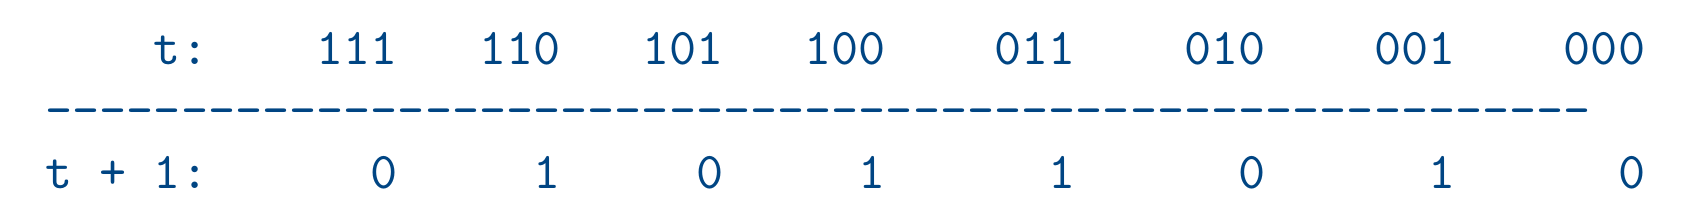
\includegraphics[width=0.5\textwidth]{media/1dimca.png}
    \caption{Egydimenziós sejtautomata egyik féle szabálya. A felső sor megdja a lehetséges kialakuló helyzeteket, az alsó sorban pedig megszabhatjuk, milyen állapotban legyen a központi cellánk a következő lépésben. } 
    \label{fig:1dimca}
    \end{center}
\end{figure}

Összességében tehát $2^8 = 256$ féle klünböző szabályt tudunk megalkotni. A \ref{fig:1dimca}. ábrán látott szabályt a 90-esnek nevezik (rule 90), ugyanis a kialakuló állapotokat binárisnak tekintve (01011010), ha átírjuk azt decimálissá, 90-et kapunk ($Bin 01011010 = Hex 90$). 

Wolfram tanulámnyozta ezt a fajta sejtautomatát, és a hosszútávú viselkedésüket tekintve az alábbi négy csoportra tudta osztani a szabályokat:

\begin{itemize}
\item \textbf{Határponti viselkedés (limit point behaviour):} sejtek értékei egy meghatározott értékhez tartanak, mely a kezdeti állapottól független,
\item \textbf{Határciklus (limit cycle behaviour):} stabil (időben) periodikus mintázat jön létre,
\item \textbf{Kaotikus viselkedés:} a sejt állapotának változása nem követ semmi struktúrát, kaotikus viselkedés jön létre,
\item \textbf{Komplex viselkedés:} komplex és lokális mozgó mintázatok jönnek létre.
\end{itemize}

\subsection{Conway életjátéka}

1970-ben John Conway matematikus alkotta meg a sejtautomaták azon csoportját, melyben egy 2 dimenziós négyzetrács van, a sejt bináris (élő - 0, halott - 1), és a sejt következő állapotát csak az életben lévő szomszédok száma határozza meg. Továbbá, \textit{Moore szomszédokat} veszünk, azaz megengedjük a diagonális átmenetet is, tehát egy sejtnek 8 szomszédja lesz -- az eredeti Neumann-féle sejtautomaták \textit{Neumann szomszédokat} használtak, ahol a diagonál nem volt megengedett, tehát 2 dimenzióban is csak 2 szomszédja volt egy sejtnek.\\
Ekkor szintén lehet definiálni szabályokat, és értelmezni egy bináris kódot: például a $000011100$ kódot úgy kell értelmezni, hogy alárakjuk az életben lévő szomszádok számát ($012345678$). A kód alapján, élő lesz (marad) a sejt, ha az életben lévő szomszédjainak a száma 4, 5 vagy 6, minden más esetben halott. Értelemszerűen, a sejt saját állapotától is függhet a jövője, amellyel a szabályokat Ezzel az élet különöző modelljeit tudjuk rekonstruálni.  

\subsection{Gáz szimulálása rácson}
Egy nagyon effektív modellt publikált U. Frisch et al. 1986-ban a kétdimenziós Navier-Stokes egyenletek alapján. Ennek a modellnek a főbb jellemzői:

\begin{itemize}
\item \textbf{Hatszögrács:} A hexagonális szimmetria elengedhetetlen ahhoz, hogy elég szabadsági fok legyen a forgásszimmetriának, így biztosítva a perdületmegmaradást.
\item \textbf{Sűrűség:} Minden cellának maximum 6 db $m=1$ tömegű részecskéje lehet, így a sűrűség 7 különböző értéket vehet fel.
\item \textbf{Szabad áramlás (Euler):} a szabad áramlás létrejöttét az alábbi szabályok segítik elő:
\begin{itemize}
\item Sebesség: minden részecskének 6 lehetséges irányú sebessége lehet, azonban egy időlépés alatt csak egy cellát mozdulhat el. 
\item Sebesség egy cellán belül: az egy cellán belül lévő részecskéknek csakis különböző irányú sebességei lehetnek -- két részecske nem akarhat ugyanoda menni.
\end{itemize}
\item \textbf{Viszkozitás (Navier-Stokes):} A viszkozitás létrejöttét	az ütközési szabályok biztosítják: ha egy sejtre 2, 3 vagy 4 részecske pályázik, azok úgy változtatják majd a sebességüket, hogy az összimpulzus megmaradjon. Ilyen ütközésekre példa a \ref{fig:hexalattice}. ábra.

\end{itemize}

	
\begin{figure}[H]
    \begin{center}
    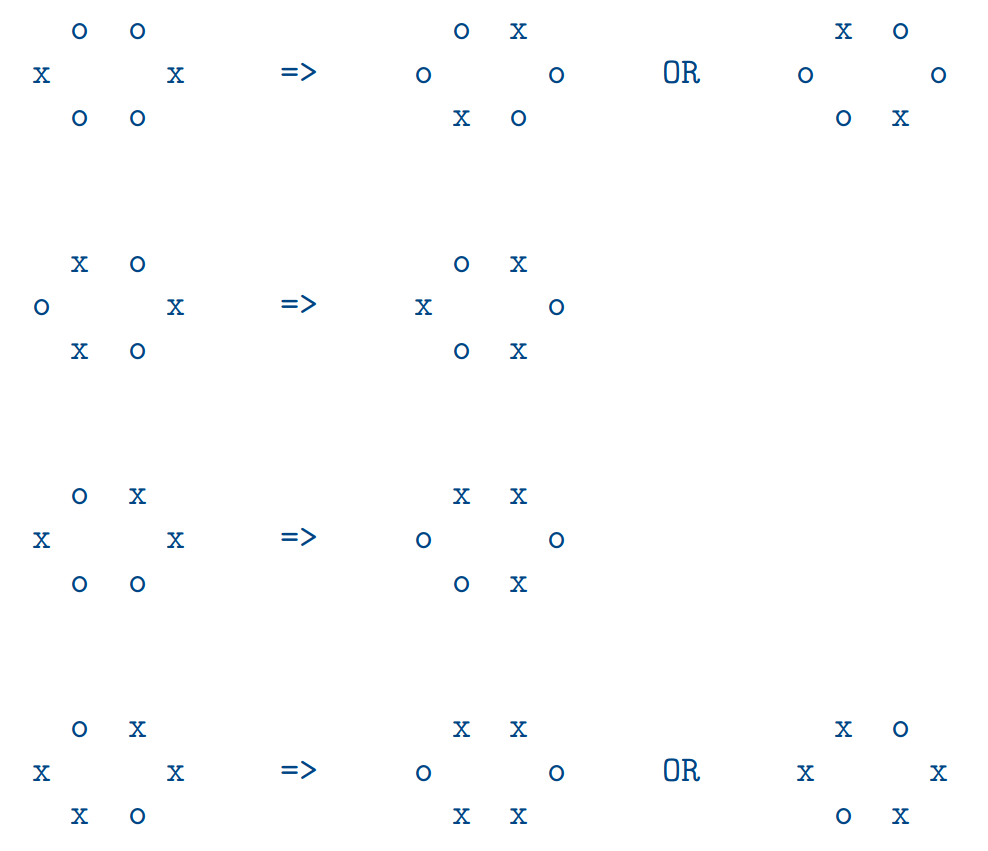
\includegraphics[width=0.5\textwidth]{media/hexalattice.png}
    \caption{Kétdimenziós hatszográcson történő ütközések lehetséges kimenetelei. Mindenhol az $X$ jelöli a részecskét, és a közepe felé haladnának. Az első és negyedik esetben a két választás egyenértékű. Ha az irányt véletlenszerűen választjuk ki, a rendszer sztochasztikussá válhat. Akkor tudjuk megtartani a rendszert determinisztikusnak, ha nem választunk kitüntetett irányt, mert így nem törik meg a királis szimmetria sem.}
    \label{fig:hexalattice}
    \end{center}
\end{figure}



\subsection*{Források} 
Fraktálokat Palla Gergely előadásjegyzete alapján: \url{http://pallag.web.elte.hu/fractals/}, a sejtautomatákat pedig Csabai István jegyzete alapján: \url{csabai.web.elte.hu/http/szamszim/lecture7/topic6-lec1.pdf} készítettem.
 

\bibliographystyle{plain}
\bibliography{references}

\end{document}
